\documentclass[slovak]{ExcelAtFIT}

%--------------------------------------------------------
%	REVIEW vs. FINAL VERSION
%--------------------------------------------------------

\ExcelFinalCopy

%--------------------------------------------------------
%	PDF CUSTOMIZATION
%--------------------------------------------------------

\hypersetup{
	pdftitle={Mobilná aplikácia pre akvizíciu a úpravu HDR fotografií},
	pdfauthor={Patrik Michalák},
	pdfkeywords={HDR, Spracovanie Obrazu, Mapovanie Tónov, Mobilná Aplikácia}
}

%--------------------------------------------------------
%	ARTICLE INFORMATION
%--------------------------------------------------------

\ExcelYear{2018}

\PaperTitle{Mobilná aplikácia pre akvizíciu a úpravu HDR fotografií}

\Authors{Patrik Michalák*}
\affiliation{*%
  \href{mailto:xmicha65@stud.fit.vutbr.cz}{xmicha65@stud.fit.vutbr.cz},
  \textit{Fakulta informačních technologií Vysokého učení technického v Brně }}

\Keywords{HDR --- Spracovanie Obrazu --- Mapovanie Tónov --- Mobilná Aplikácia}

\Supplementary{\href{https://youtu.be/60rHqo7lZIQ}{Demonštračné Video}}

%--------------------------------------------------------
%	ABSTRACT and TEASER
%--------------------------------------------------------

\Abstract{
	Cieľom tejto práce je návrh a implementácia mobilnej aplikácie pre akvizíciu, spracovanie, zobrazenie
	a úpravu HDR fotografií. V riešení bola použitá metóda generovania HDR obsahu kombinovaním LDR snímok
	s rôznou hodnotou času expozície. Vytvorené riešenie poskytuje užívateľovi mobilnú aplikáciu pre prácu
	s HDR fotografiou, štyri metódy mapovania tónov a rôzne nástroje, ktoré užívateľ pri práci potrebuje.
}

\Teaser{
	\TeaserImage{teaser}
}

%--------------------------------------------------------
%--------------------------------------------------------
\begin{document}

\startdocument

%--------------------------------------------------------
%	ARTICLE CONTENTS
%--------------------------------------------------------

\section{Úvod}

Okolie, ktoré vnímame, má vysoký dynamický rozsah svetla a farieb. Tmavé miesta bez osvetlenia neobsahujú takmer žiaden jas a naopak
scéna zameraná na zdroj svetla obsahuje priveľmi veľa jasu. Ľudské oko je schopné prispôsobiť sa takýmto zmenám a pozorovať detaily
aj na scéne s rozmanitým rozsahom jasu. Fotoaparát však nemá taký cit ako človek a dokáže zachytiť snímky len s určitou
hodnotou expozície. Preto sa digitálne fotoaparáty pokúšajú odhadnúť osvetlenie a automaticky nastaviť čas expozície tak, aby mal
najdôležitejší aspekt scény čo najlepšií dynamický rozsah a jas miest, ktoré sú príliš tmavé alebo naopak príliš svetlé, je orezaný
na~hodnoty 0 a 255. Tento problém rieši HDR fotografia, avšak nie veľa bežných užívateľov si je vedomých, čo to vlastne HDR fotografia
znamená a ako sa s ňou pracuje.

HDR umožňuje zachytiť veľkú časť rozsahu jasu reálneho sveta a následnú prácu s týmito dátami. Existuje viacero mobilných aplikácií,
ktoré ponúkajú vytvorenie a spracovanie HDR fotografie. Veľa verejne dostupných aplikácií však používa iba filter aplikovaný na jednu
fotografiu, ktorý zvýši kontrast farieb a detaily a tým sa snaží opticky vytvoriť efekt HDR. Na druhej strane sú aplikácie, ktoré
vytvárajú HDR fotografiu skladaním série snímok s rôznymi nastavenia- mi expozície. Tieto aplikácie však poväčšine užívateľo- vi neposkytujú
dostatočne záživné užívateľské rozhranie, majú pre užívateľa veľmi obmedzené možnosti, alebo sa s nimi ťažko a neintuitívne pracuje.

Zameraním tejto práce je vytvoriť aplikáciu, ktorá by riešila nielen problémy generovania a spracovania HDR obsahu, ale zamerala sa aj na
interakciu s užívateľom a poskytla mu viac možností ako bežná aplikácia. Každá scéna je niečim výnimočná a jednoduché východzie nastavenia
hodnôt parametrov nedosiahnú vždy uspokojivé výsledky.

%--------------------------------------------------------
%--------------------------------------------------------
\section{Generovanie a spracovanie HDR}
\label{sec:Theory}

Je veľmi obtiažne zachytiť scénu, kde sú svetlé miesta mnohonásobne jasnejšie ako tmavé miesta. Inak povedané, takáto scéna má vysoký
dynamický rozsah.
V súčasnosti existujú 3 metódy vytvárania HDR obsahu \cite{ZakladyHDR}:
\begin{itemize}
    \item kombinovaním LDR snímok s rôznou hodnotou času expozície,
    \item zachytenie scény špecializovaným hardvérom,
		\item vytváranie virtuálnych prostredí.
\end{itemize}

Kombinovanie viacerých snímok scény s rôznou hodnotou expozície je pre svoju dostupnosť a nenároč- nosť najviac využívanou metódou.
Takto zachytíme detaily od najtmavšej, až po najsvetlejšiu oblasť.

%--------------------------------------------------------
\subsection{Generovanie HDR}
\label{sec:Theory-Generate}

Digitálne fotoaparáty majú všeobecnú funkciu nazývanú krivka odozvy fotoaparátu (CRF\footnote{Camera Response Function}).
Predtým, ako budeme generovať HDR obsah, je potrebné vyjadriť túto krivku odozvy snímača zariadenia.
Krivku získame minimalizovaním kvadratickej objektívnej funkcie \cite{Debevec}:
\begin{equation}
	\mathcal{O} = 
	\sum_{i=1}^{N}
	\sum_{j=1}^{P}
	[g(Z_{ij}) - \ln E_{i} - \ln \Delta t_{j}]^{2}
	+ \lambda
	\sum_{z=Z_{min} + 1}^{Z_{max} - 1}
	g''(z)^{2}
\end{equation}
kde $P$ je počet obrázkov s rozličnou expozíciou, $N$ je počet pixelov v jednom obrázku, $Z_{ij}$ je hodnota pixelu na indexe $i$ v obrázku $j$,
$Z_{min}$ a~$Z_{max}$ sú hodnoty minima a maxima, ktoré môže pixel nadobudnúť a $\Delta t_{j}$ je expozičný čas pre $Z_{ij}$.
Druhý term zabezpečuje plynulosť funkcie $g$. Hodnota $\lambda$ je váha plynulosti relatívna 
k prvému termu a je zvolená podľa množstva šumu očakávaného v $Z_{ij}$.
$w(Z_{ij})$ je váhová funkcia odstraňujúca presahujúce hodnoty \cite{Debevec}:
\begin{equation}
  w(z)=
  \begin{cases}
    z - Z_{min}, & \text{pre}\ z \leq \frac{1}{2}(Z_{min} + Z_{max}) \\
    Z_{max} - z, & \text{pre}\ z > \frac{1}{2}(Z_{min} + Z_{max})
  \end{cases}
\end{equation}
pomocou ktorej dosiahneme, že hodnoty v okolí $Z_{mid}$ budú mať väčšiu váhu ako hodnoty v okolí $Z_{min}$ a $Z_{max}$. $Z_{mid}$ je prostredná
hodnota rozsahu hodnôt pixelu, vyjadrená ako $Z_{mid} = \frac{1}{2}(Z_{min} + Z_{max})$.

Ak už máme vyjadrenú krivku odozvy $g$, vieme ju spolu s váhovou funkciou použiť na prepočet hodnoty pixelu na relatívnu hodnotu žiarenia
$E_{i}$ \cite{Debevec}:
\begin{equation}
    \ln E_{i} = 
    \frac{
        \sum_{j=1}^{P}
        w(Z_{ij})(g(Z_{ij}) - \ln \Delta t_{j})
    }{
        \sum_{j=1}^{P}
        w(Z_{ij})
    }
\end{equation}

%--------------------------------------------------------
\subsection{Zobrazovanie HDR obsahu}
\label{sec:Theory-TMO}

Vzhľad scény závisí od úrovne osvetlenia a rozsahu kontrastu \cite{HDRI}. Za jasného dňa vyzerá scéna viac farebne a kontrastnejšie. Pre reprodukovanie
presného vizuálne- ho vzhľadu takejto scény nestačí iba jednoduchá kompresia, aby sa úroveň intenzity a rozsah kontrastu prispôsobil limitom zobrazovacieho
média.

Reprodukcia vizuálneho vzhľadu je primárnym cieľom pre mapovanie tónov.
Mapovanie tónov je proces prevodu obrazu s vysokým dynamickým rozsahom na 8-bitový obraz pre farebný kanál, s cieľom zachovať čo najväčšie množstvo detailov.

Metódy mapovania tónov môžeme rozdeliť na dva základné typy:
\begin{description}
    \item [Globálne operátory] (priestorovo jednotné) sú nelineár- ne funkcie založené na svetelných a iných
    globál- nych premenných obrazu. \cite{AHDR}
    \item [Lokálne operátory] (priestorovo sa meniace) sú nelineárnej funkcie, ktorých parametre sa menia
    v každom pixeli podľa vlastností získaných z~okoli- tých oblastí. \cite{AHDR}
\end{description}

Aplikáciou implementované metódy mapovania tónov sú:
\begin{description}
	\item [Bilaterálny filter] - metóda sa pokúša zobraziť obrazy HDR
    rozložením obrazu na základnú vrstvu a vrstvu detailov. V základnej vrstve je kontrast skomprimovaný
		bilaterálnym filtrom, ktorý chráni hrany. \cite{TMODurand}
	\item [Fotografická reprodukcia] - tento operátor simuluje techniku "dodging and burning", ktorá bola použí- vaná
    v počiatkoch fotografie a dovoľuje vytvárať rozličné expozície naprieč fotografiou. Operátor
		obsahuje aj jednoduchšiu globálnu verziu. \cite{TMOReinhard}
	\item [Logaritmické mapovanie] - metóda redukuje pomer kontrastu logaritmickou kompresiou hodnôt jasu,
    napodobňujúc ľudské vnímanie svetla. \cite{TMODrago}
	\item [Perceptuálny rámec pre kontrastné spracovanie] - \hfill \\ metóda vytvára rámec pre spracovanie obrazu
		v priestore vizuálnej odozvy, v ktorej kontrastné hodnoty priamo korelujú so svojou viditeľnosťou
		v obraze. \cite{TMOMantiuk}
\end{description}

%--------------------------------------------------------
%--------------------------------------------------------
\section{Návrh a Implementácia Aplikácie}
\label{sec:Implement}

Výber technológií pre implementáciu časovo a priestoro- vo náročných algoritmov je dôležitá a často 
náročná časť práce. Táto práca bude zameraná na vytváranie HDR fotografie na platforme Android.
Pre riešenie náročných matematických a grafických operácií je použitá knižnica OpenCV.

%--------------------------------------------------------
\subsection{Užívateľské rozhranie}
\label{sec:Implement-UI}

Aplikácia sa zameriava na širokú škálu užívateľov - od náročného fotografa až po technicky neskúsenú
osobu, snažiacu sa vytvoriť čo najdôverihodnejší záber scény. Preto by mala aplikácia minimalistickým 
a intuitívnym spôsobom ponúkať všetky potrebné nástroje a možnosti, ktoré môže užívateľ použiť.

\begin{figure}[t]
  \centering
	
\includegraphics[width=0.3\linewidth]{sketch/sketch-home}
	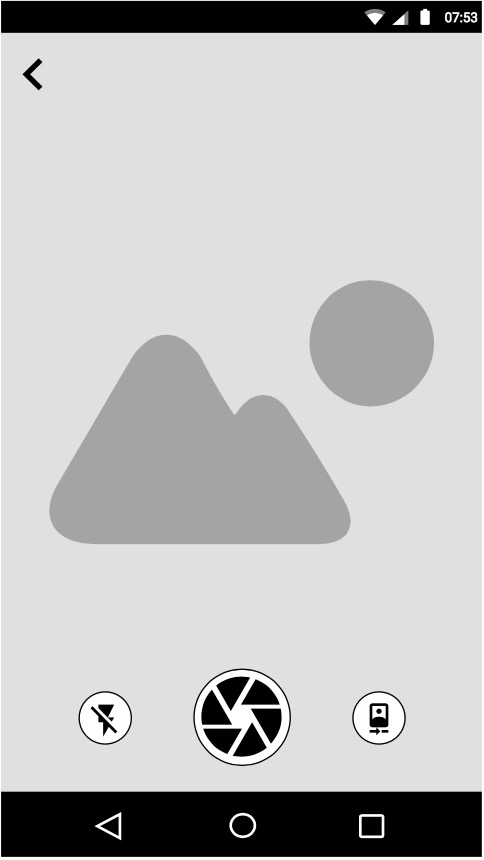
\includegraphics[width=0.3\linewidth]{sketch/sketch-capture}
	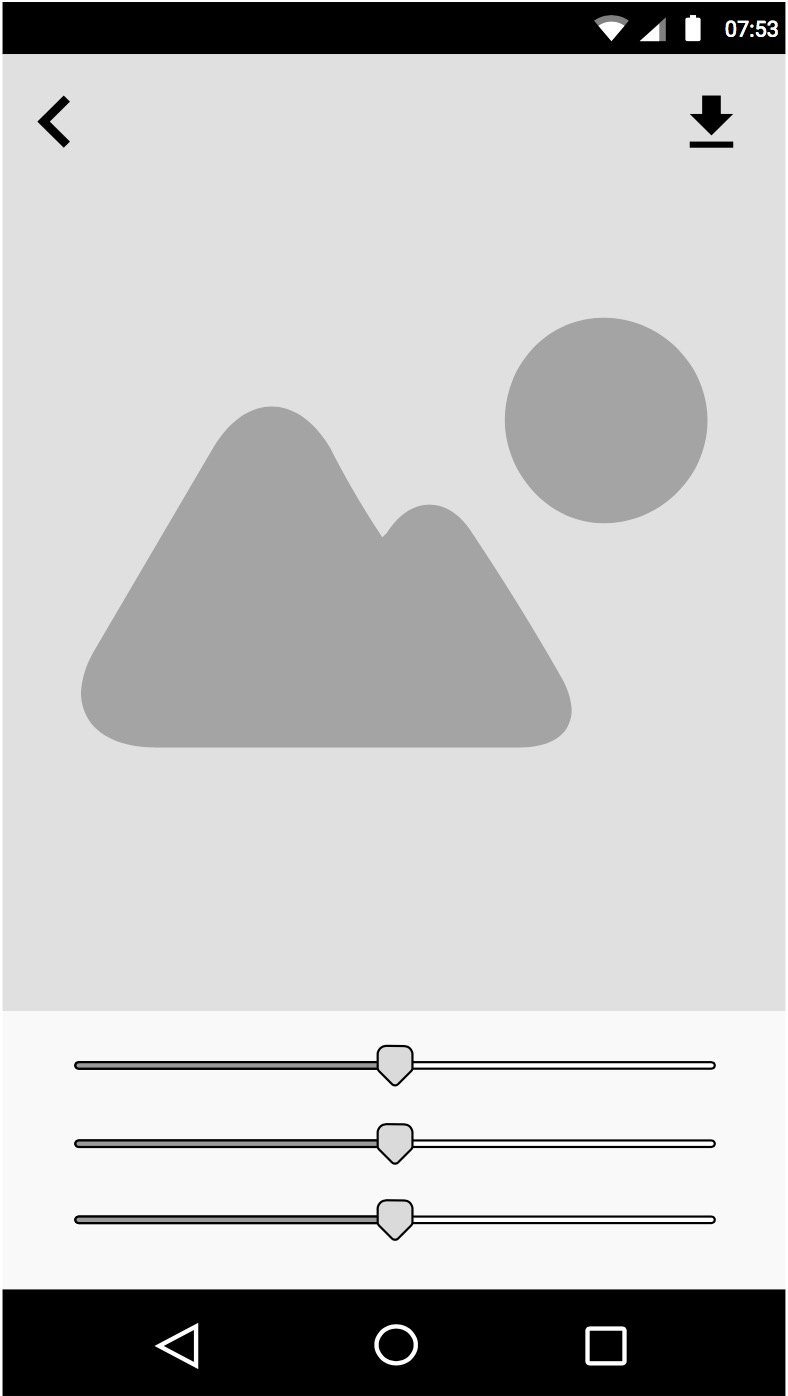
\includegraphics[width=0.3\linewidth]{sketch/sketch-edit}
  \caption{Návrh užívateľského rozhrania}
  \label{fig:SketchScreens}
\end{figure}

Domovská obrazovka je príkladom toho, že užívateľ môže mať všetko čo potrebuje,
bez zbytočného zdĺhavé- ho hľadania. Na vytvorenie HDR fotografie potrebujeme buď zachytiť aktuálnu scénu
fotoaparátom, alebo načítať súbor s HDR obsahom. Po zachytení scény na~fotografiu, alebo načítaní HDR obsahu a~po spracovaní 
tohoto obsahu, má užívateľ na výber z rôznych techník mapovania tónov. Po výbere jednej z nich je
užívateľovi poskytnutá možnosť upravovania fotografie do výslednej podoby 
pomocou prehľadnej ponuky nástrojov. Jednotlivé parametre sú spočiatku nastavené na vhodné východzie 
hodnoty, ktoré je možné po úpravach zresetovať. Na záver je možné výsledok uložiť do galérie.

%--------------------------------------------------------
\subsection{Snímanie}
\label{sec:Implement-Capturing}

Aplikácia generuje HDR obsah kombinovaním LDR fotografií s rôznou hodnotou času expozície.
Snímanie fotografií je implementované nad aplikačným rozhraním
Camera2\footnote{\url{https://developer.android.com/reference/android/hardware/camera2/package-summary.html}}
operačného systému Android.

Pre zobrazovanie scény v reálnom čase zobrazujeme na výstup stream záberov scény, ktorý dosiahneme nastavením
opakovaného požiadavku o snímanie. Pri zobrazovaní náhľadu využijeme automatické nastavenia
parametrov. Do vytvoreného požiadavku o~sní- manie scény vložíme callback, kde odchytíme objekt s meta informáciami.
Tento objekt obsahuje hodnoty konfigurácie snímača zariadenia, po vytvorení posledného snímku. Z tejto
konfigurácie následne získavame hodnoty expozície, ISO, clony a korekcie farieb, ktoré sú automaticky zvolené
snímačom. Hodnoty ukladáme do premenných, ktoré neskôr použijeme v manuálnom režime snímania.

V okamihu, keď užívateľ stlačí tlačítko pre snímanie scény, je potrebné vytvoriť sériu záberov s manuálne nastavenými
hodnotami parametrov. Najdôležitejším parametrom je dĺžka expozičného času, počas ktorého je snímač vystavený svetlu
z prostredia scény.

\subsection*{Nastavenie času expozície}

Každý snímač zariadenia obsahuje súbor vlastností a nastavení, ku ktorým pristupujeme pomocou
objektu \texttt{CameraCharacteristics} \cite{Android}. Odtiaľ získame aj rozsah povoleného expozičného
času snímača. V~oka- mihu, keď nastane stav manuálneho snímania scény, potrebujeme vytvoriť zoznam
vybraných expozičných časov, ktorých strednou hodnotou bude hodnota automatickej expozície. Povolený
rozsah expozičného času však nemusí umožňovať, aby prostrednou hodnotou bola práve táto hodnota.
Pre riešenie týchto problémov bol vytvorený algoritmus, ktorý hľadá vhodné hodnoty expozičných
časov v povolenom rozsahu (obr. \ref{fig:Exposures}).

Algoritmus vytvára zoznam hodnôt geometrického radu v tvare $2^{n}$ $ns$ v povolenom rozsahu.
V tomto zozname sa zvolí hodnota najbližia hodnote automatickej expozície ako prostredná hodnota
a vo zvolenom kroku sa striedavo hľadajú hodnoty nižšie od strednej hodnoty a hodnoty vyššie.
Algoritmus končí, ak konečný zoznam obsahuje zvolený počet expozičných časov, alebo ak nie je
možné nájsť ďalšiu hodnotu.

\begin{figure}[ht!]
  \centering
  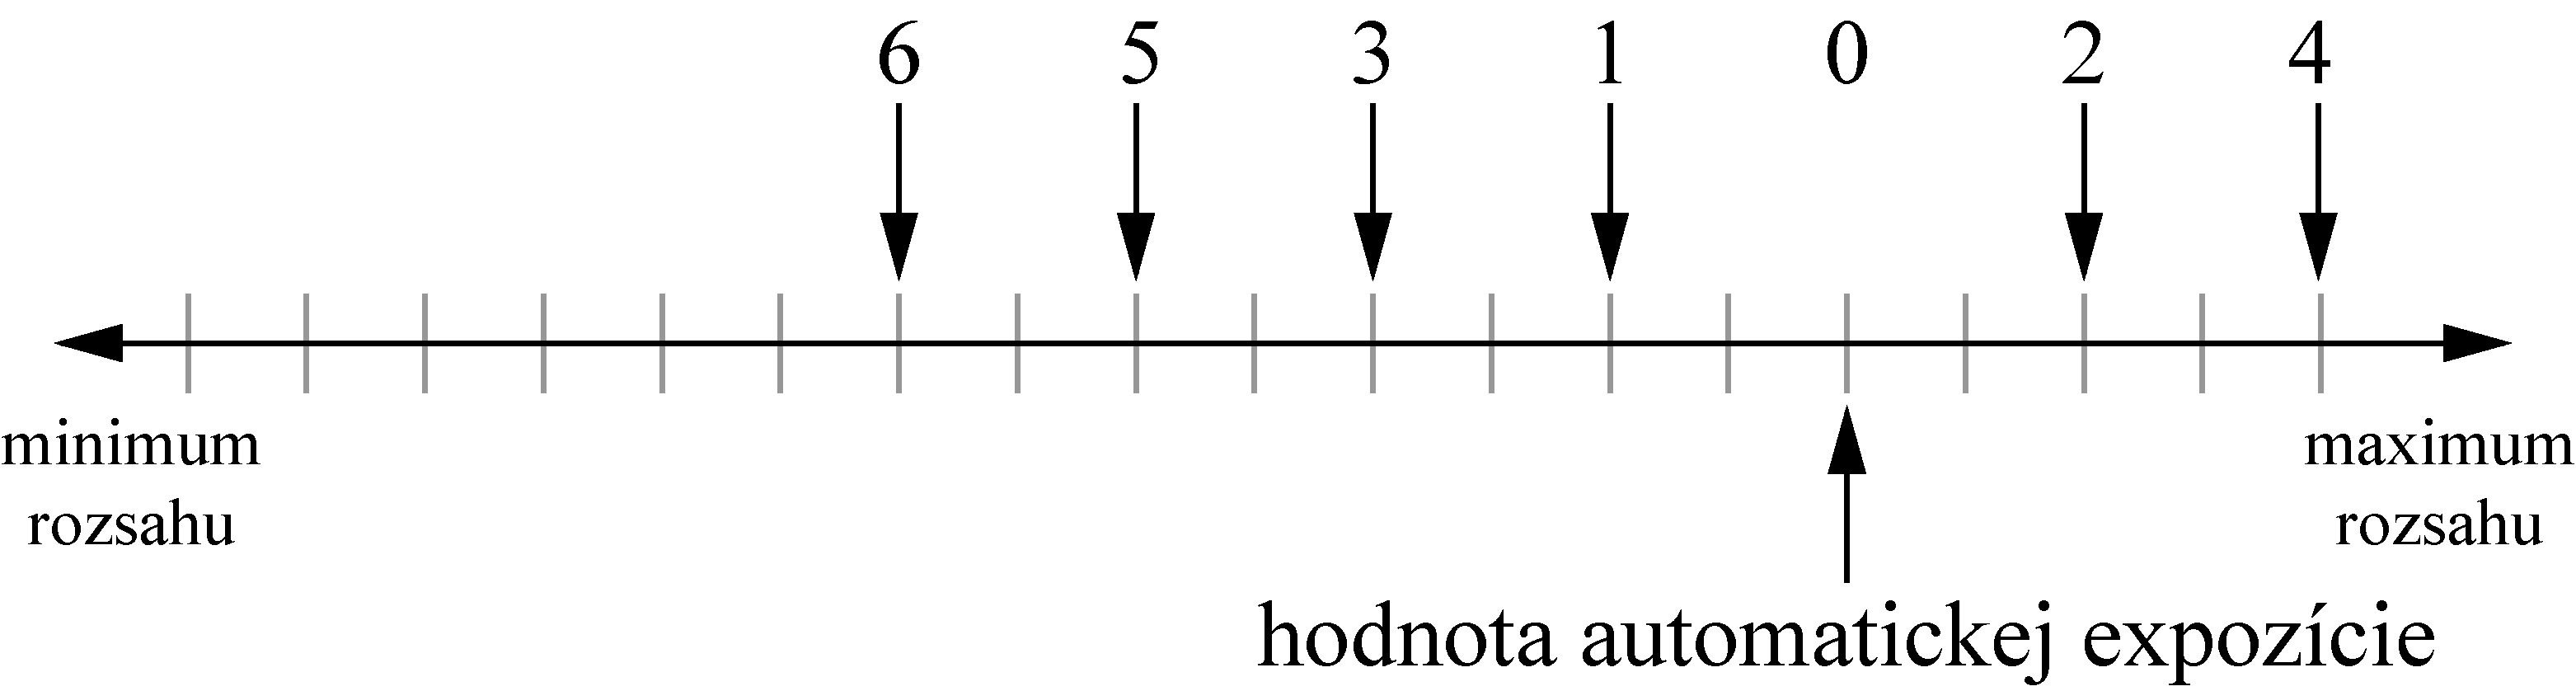
\includegraphics[width=1\linewidth]{expoSelector2}
  \caption{Vyhľadávanie vhodných hodnôt expozície s krokom 2 (čísla zobrazujú poradie nájdených hodnôt)}
  \label{fig:Exposures}
\end{figure}

\subsection*{Zarovnanie}

Nezarovnanie snímok použitých pri vytváraní HDR obrazu môže mať za následok artefakty nazývané ghosting (duchovia), 
ktoré majú vplyv na výsledný obrázok. Ghosting nastáva aj v prípade, že sa na statickej scéne nachádza objekt, 
ktorý je voči scéne v pohybe.

Pre zarovnanie vytvorených snímok je použitá metóda Median Threshold Bitmap \cite{Align}. Vstupom metódy
je zoznam vytvorených snímok. Podľa histogramu jasu obrázkov sa určí 8-bitová hodnota mediánu a vytvoria sa MTB obrazy,
kde každý pixel, ktorý je jasnejší než medián, má hodnotu 1 a~v~opačnom prípade hodnotu 0. Rýchlosť tejto
metódy spočíva vo využívaní bitových operácií nad MTB obrazmi. Výstupom metódy je zoznam zarovnaných snímok.

%--------------------------------------------------------
\subsection{Generovanie HDR obsahu}
\label{sec:Implement-Generate}

Pred generovaním samotného HDR obsahu si musíme vyjadriť krivku odozvy fotoaparátu a to riešením kvadra- tickej
objektívnej funkcie z podkapitoly \ref{sec:Theory-Generate}. Teoreticky by sa na riešene tejto rovnice mohol vziať
každý pixel, každej expozície, ale to by bolo na výpočet veľmi časovo a priestorovo náročné. My však nepotrebujeme
všetky dostupné pixely. Ak máme $P$ fotografií po $N$ pixelov, výsledná intenzita žiarenia $E_{i}$ bude mať $N$ hodnôt
a krivka odozvy $g$ $(Z_{max} - Z_{min})$\cite{Debevec} hodnôt. Tieto hodnoty však musíme vhodne vybrať zo sekvencie
expozícii.
Medzi dostupné metódy výberu pixelov pre získanie krivky odozvy môžeme zaradiť:
\begin{itemize}
  \item výber pixelov pomocou histogramu,
  \item pravidelne usporiadané pixely,
  \item náhodný výber pixelov (implementované\\v aplikácii).
\end{itemize}

Keďže aplikácia pracuje s farebnými obrázkami, musíme vyjadriť krivku odozvy $g$ pre každý farebný kanál
(obr. \ref{fig:CameraCurve}). Aplikácia implementuje riešenie rovnice na základe ukážky \texttt{MATLAB}
kódu \cite{Debevec}. Kód bol
debugovaný pomocou voľne šíriteľného softvéru GNU Octave\footnote{\url{www.gnu.org/software/octave/}}
a následne implementovaný v Jave. V závere algoritmu je potrebné vykonať dekompozíciu vytvorených matíc. Dekompozícia
je realizovaná pomocou metódy SVD\footnote{Singular-value Decomposition}, z knižnice OpenCV.

\begin{figure}[t]
  \centering
  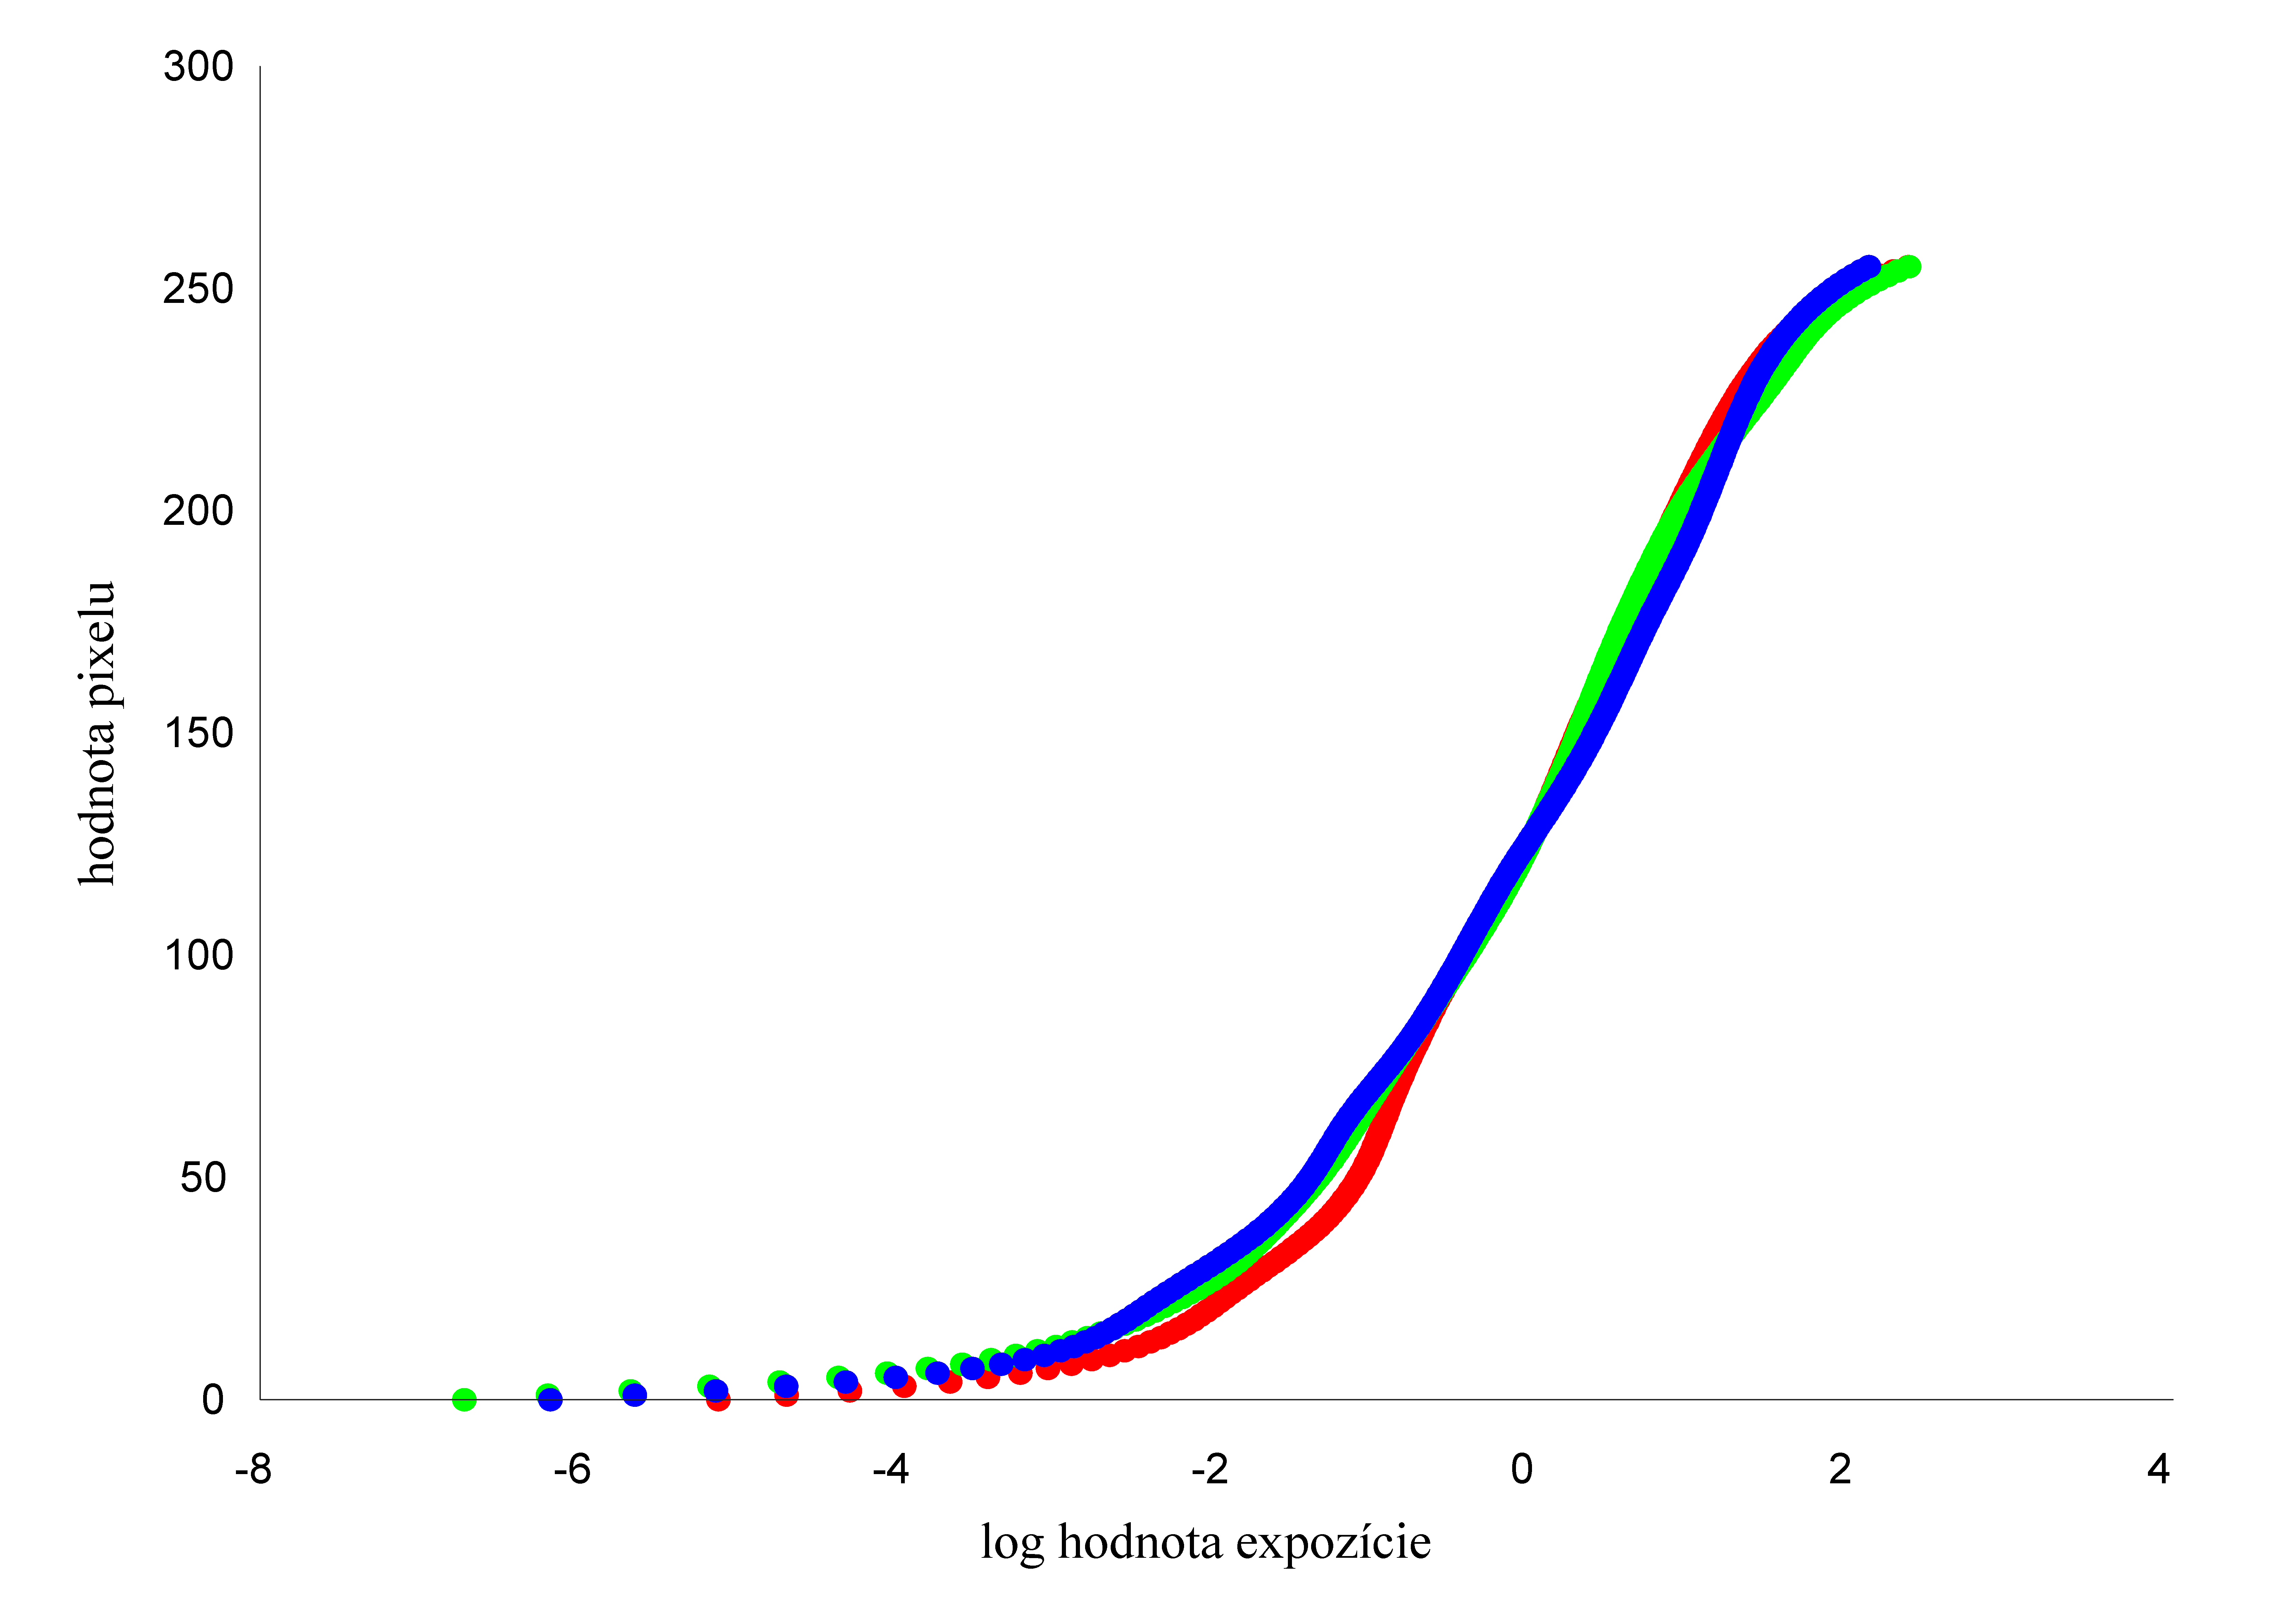
\includegraphics[width=0.8\linewidth]{cameraCurve}
  \caption{Graf CRF kriviek farebných kanálov}
  \label{fig:CameraCurve}
\end{figure}

Na získanie HDR obsahu potrebujeme vyjadriť $\ln E_{i}$ (podkapitola \ref{sec:Theory-Generate}) pre každý pixel
a každý farebný kanál.

%--------------------------------------------------------
\subsection{Prevod HDR obsahu na LDR}
\label{sec:Implement-TMO}

Dostali sme sa do stavu, kedy máme vytvorený HDR obsah z $n$ nasnímaných fotografií. Tento obsah je nutné vhodne užívateľovi prezentovať.
Po vytvorení HDR obsahu sa preto zobrazí obrazovka, na ktorej je zoznam implementovaných operátorov mapovania tónov s ich náhľadom.
Jednotlivé operátory mapovania tónov sú implementované pomocou knižnice OpenCV, ktorá poskytuje globálne operátory \texttt{Reinhard},
\texttt{Drago}\\a lokálne operátory \texttt{Durand} a \texttt{Mantiuk}.

Ak si užívateľ vyberie jeden zo zoznamu ponúka- ných operátorov mapovania tónov, zobrazí sa obrazovka pre editovanie parametrov operátora
pomocou posuvníkov. Okrem posuvníkov obsahuje obrazovka náhľadový obrázok a tlačítka pre uloženie HDR obsahu a výslednej LDR fotografie,
tlačítko pre resetovanie nastavení na východzie hodnoty a tlačítko pre otočenie náhľadového obrázku.

\subsection*{Zmenšenie náhľadového obrázka}

Operátory mapovania tónov sa pre náhľadové obrázky aplikujú na zmenšený HDR obsah. To zaručí menšiu časovú náročnosť zobrazenia
obrazovky s operátormi mapovania tónov. Zmenšenie náhľadového obrázku je implementované pomocou metódy knižnice OpenCV, využitím
bilineárnej interpolácie. Na obrazovke vybraného operátora mapovania tónov, kde je možné modifikovať vstupné parametre algoritmu,
môže byť vďaka zmenšeniu zobrazovaný náhľad v reálnom čase bez väčších oneskorení.

%--------------------------------------------------------
\subsection{Ukladanie}
\label{sec:Implement-Storage}

V závere celého procesu vytvárania HDR fotografie musí byť užívateľ schopný uložiť si výsledok. Apli- kácia ponúka
uloženie nielen výslednej fotografie v~štan- dardnom obrazovom formáte \texttt{JPEG}, ale aj uloženie HDR obsahu 
pre neskoršiu editáciu. V tomto prípade je HDR obsah komprimovaný kódovaním 
\texttt{RGBE}\footnote{\url{https://en.wikipedia.org/wiki/RGBE_image_format}}. Ulo- ženie HDR formátu
je veľkou výhodou, ktorú nepo- núka žiadna z aplikácií prieskumu. Užívateľ sa totiž nemusí práve nachádzať
v situácii, kedy si nájde čas na vhodné prispôsobenie výsledných parametrov LDR obrazu.

Užívateľ môže k uloženým HDR súborom pristupovať kedykoľvek v obrazovke, ktorá obsahuje výpis uložených
\texttt{.hdr} súborov v zariadení užívateľa. Výber- om jedného z ponúkaných súborov sa súbor načíta a~zobrazí 
sa obrazovka pre editáciu HDR obsahu.

Pri ukladaní HDR obsahu alebo LDR výslednej fotografie je užívateľ pomocou dialógového okna vyzvaný, aby do textového
poľa vložil názov svojho nového súboru.

%--------------------------------------------------------
%--------------------------------------------------------
\begin{figure*}[t]
	\centering
	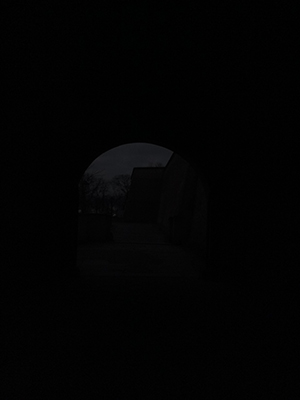
\includegraphics[width=0.086\linewidth]{series/s0}
	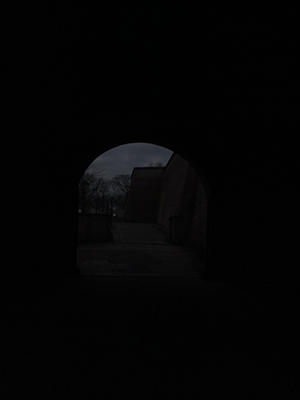
\includegraphics[width=0.086\linewidth]{series/s1}
	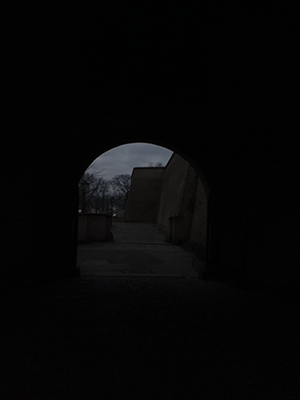
\includegraphics[width=0.086\linewidth]{series/s2}
	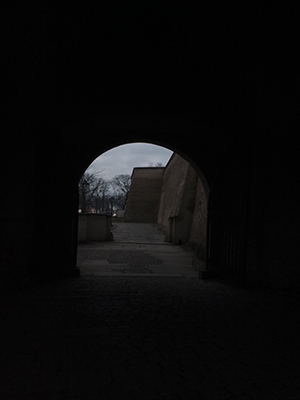
\includegraphics[width=0.086\linewidth]{series/s3}
	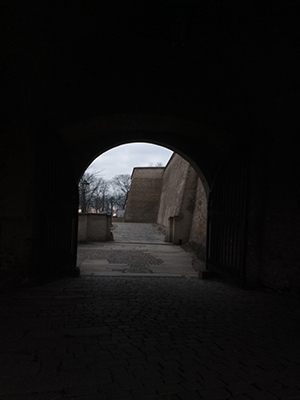
\includegraphics[width=0.086\linewidth]{series/s4}
	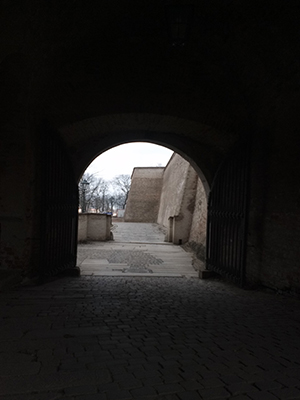
\includegraphics[width=0.086\linewidth]{series/s5}
	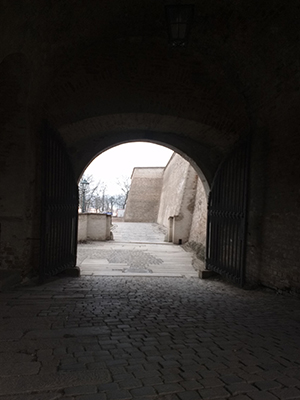
\includegraphics[width=0.086\linewidth]{series/s6}
	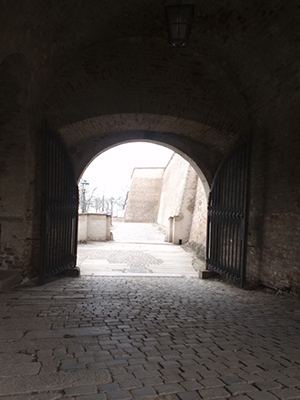
\includegraphics[width=0.086\linewidth]{series/s7}
	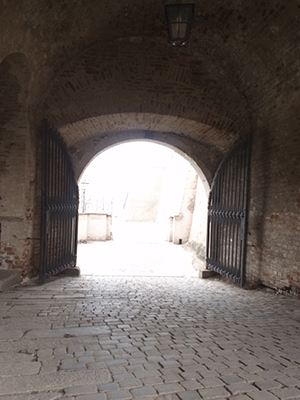
\includegraphics[width=0.086\linewidth]{series/s8}
	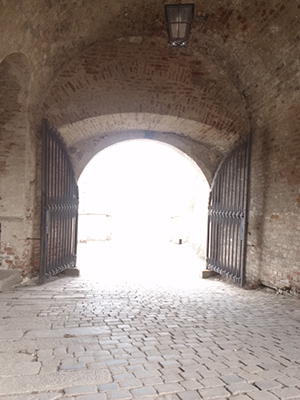
\includegraphics[width=0.086\linewidth]{series/s9}
	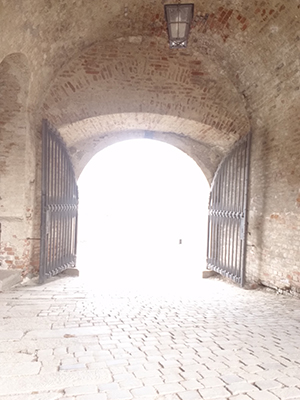
\includegraphics[width=0.086\linewidth]{series/s10}
  \caption{Séria 11 snímok scény \textit{brana} zachytených s rôznym expozičným časom}
  \label{fig:BranaSeries}
\end{figure*}

\section{Merania a Výsledky Práce}
\label{sec:Result}

Na testovanie mobilnej aplikácie bolo zachytených 6 scén. Každú scénu tvorí 11 snímok od najtmavšej po najsvetlejšiu
expozíciu. Každá scéna je význačná rôznymi, pre prácu prínosnými vlastnosťami. Pri mera- ní a porovnávaní výsledkov
sa používala primárne scéna \textit{brana} (obr. \ref{fig:BranaSeries}).

%--------------------------------------------------------
\subsection{Výsledky operátorov mapovania tónov}
\label{sec:Result-TMO}

Testované scény boli hodnotené a porovnávané pri použití rôzných nastavení pre štyri operátory mapovania tónov.
Globálne operátory \texttt{Reinhard} a \texttt{Drago} (obr. \ref{fig:GlobalTMOs}) neumožňujú na scéne s vysokým
dynamickým získať uspokojivý výsledok, kde by boli jasne viditeľné zároveň príliš tmavé a svetlé oblasti.

Jedinou užívateľom definovateľnou hodnotou ope- rátora \texttt{Drago} je hodnota skreslenia (bias). Menšie hodnoty vytvárajú
výrazne svetlejšie snímky. Pri hodnotách, ktoré sa blížia minimu rozsahu nastáva na svetlých častiach nežiadúci stav - inverzia
tónov.

Najlepšie výsledky ponúka užívateľovi lokálny operátor \texttt{Durand} (obr. \ref{fig:LocalTMOs}). Zo všetkých operátorov ponúka
užívateľovi najviac možností editovania vstupných parametrov. Pomocou nastavenia kontrastu môže užívateľ dobre definovať pomer
výsledných hod- nôt jasu a tak vytvárať obrazy verne zobrazujúce scénu alebo obrazy s umeleckým efektom. Zmenou hodnôt
bilaterálneho filtra \texttt{sigma\_color} a~\texttt{sigma\_space} užívateľ zdôrazňuje detaily scény (obr. \ref{fig:DurandUsage}).
Pri maximál- nych hodnotách bilaterálneho filtra si môžeme všimnúť halo efekt (obr. \ref{fig:DurandHalo}), spôsobený ostrým
prechodom medzi zreteľne svetlou a tmavou oblasťou.

\begin{figure}[t]
  \centering
	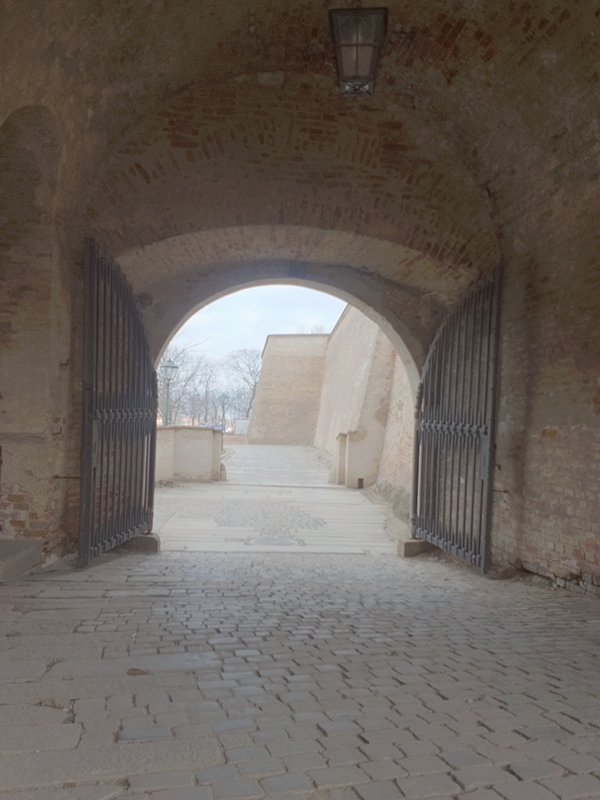
\includegraphics[width=0.49\linewidth]{tmo/rein1}
	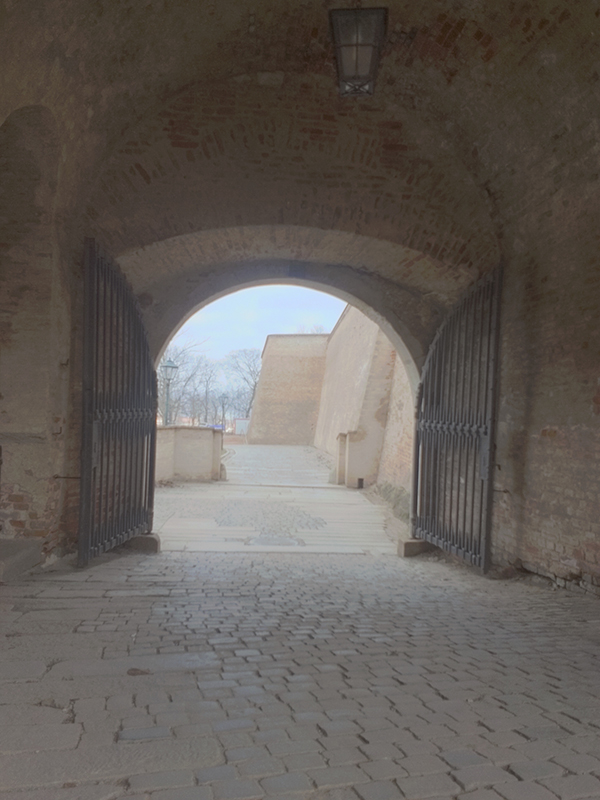
\includegraphics[width=0.49\linewidth]{tmo/drag1}
  \caption{Výsledky mapovania tónov globálnymi operátormi Reinhard \textit{(vľavo)} a Drago \textit{(vpravo)}}
  \label{fig:GlobalTMOs}
\end{figure}

\begin{figure}[t]
  \centering
	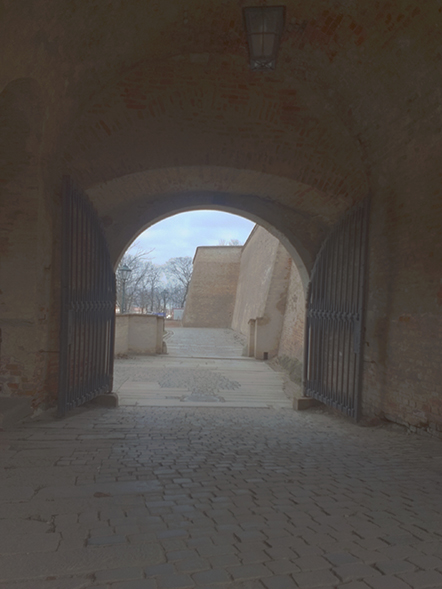
\includegraphics[width=0.49\linewidth]{tmo/man3}
	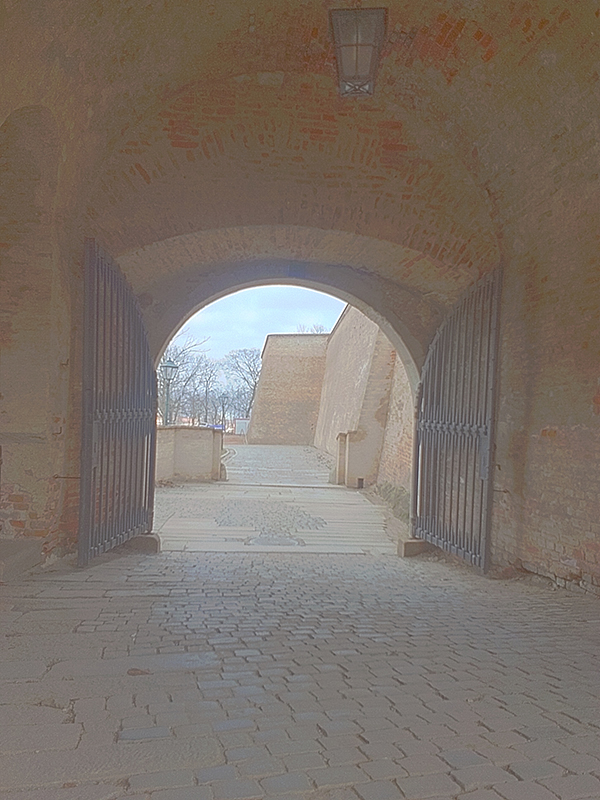
\includegraphics[width=0.49\linewidth]{tmo/dur3}
	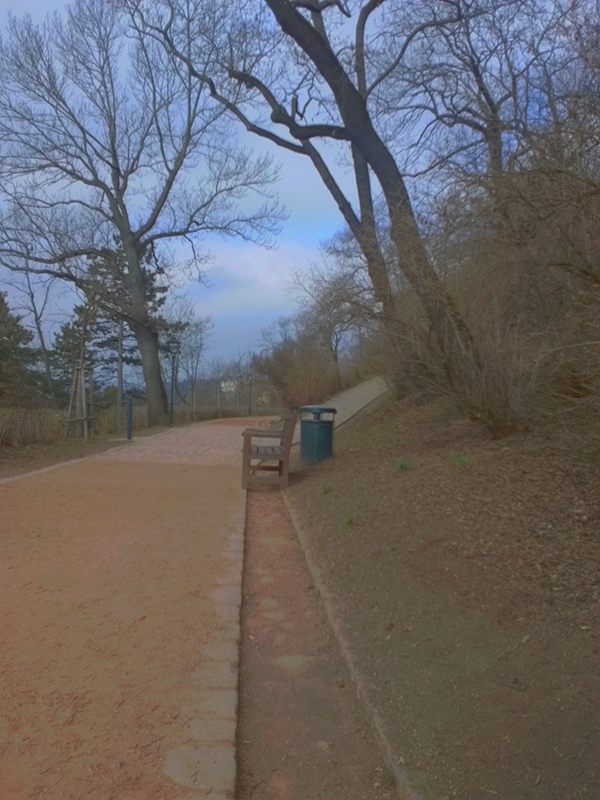
\includegraphics[width=0.49\linewidth]{tmo/man4}
	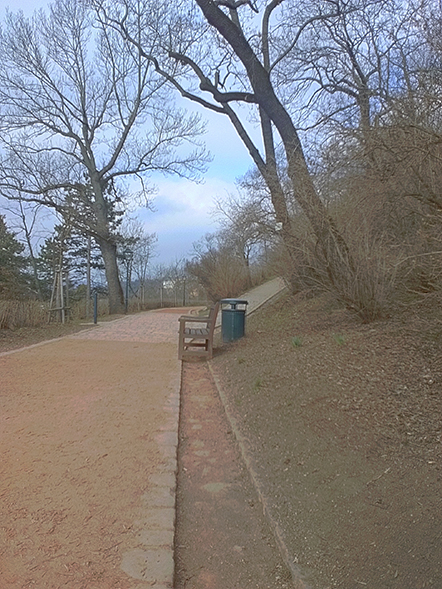
\includegraphics[width=0.49\linewidth]{tmo/durVerna2}
  \caption{Výsledky mapovania tónov lokálnymi operátormi Mantiuk \textit{(vľavo)} a Durand \textit{(vpravo)}}
  \label{fig:LocalTMOs}
\end{figure}

\begin{figure}[t]
  \centering
	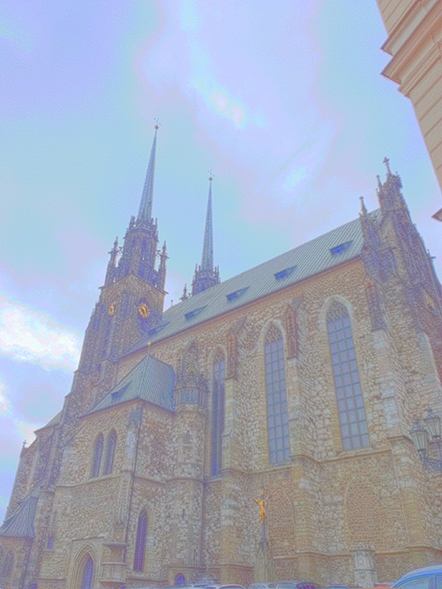
\includegraphics[width=0.49\linewidth]{tmo/durSpace1}
	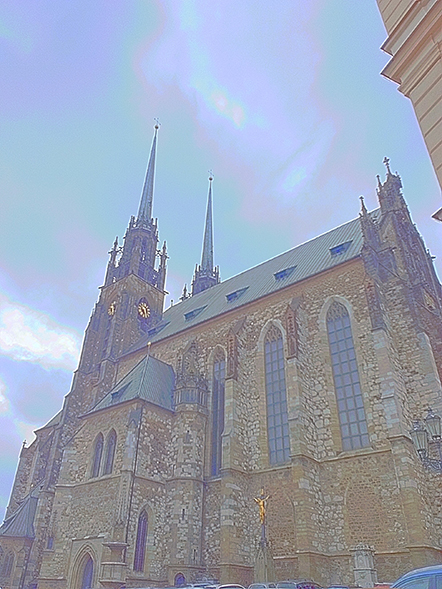
\includegraphics[width=0.49\linewidth]{tmo/durSpace2}
  \caption{Vplyv bilaterálneho filtra na detaily scény}
  \label{fig:DurandUsage}
\end{figure}

\begin{figure}[t]
  \centering
	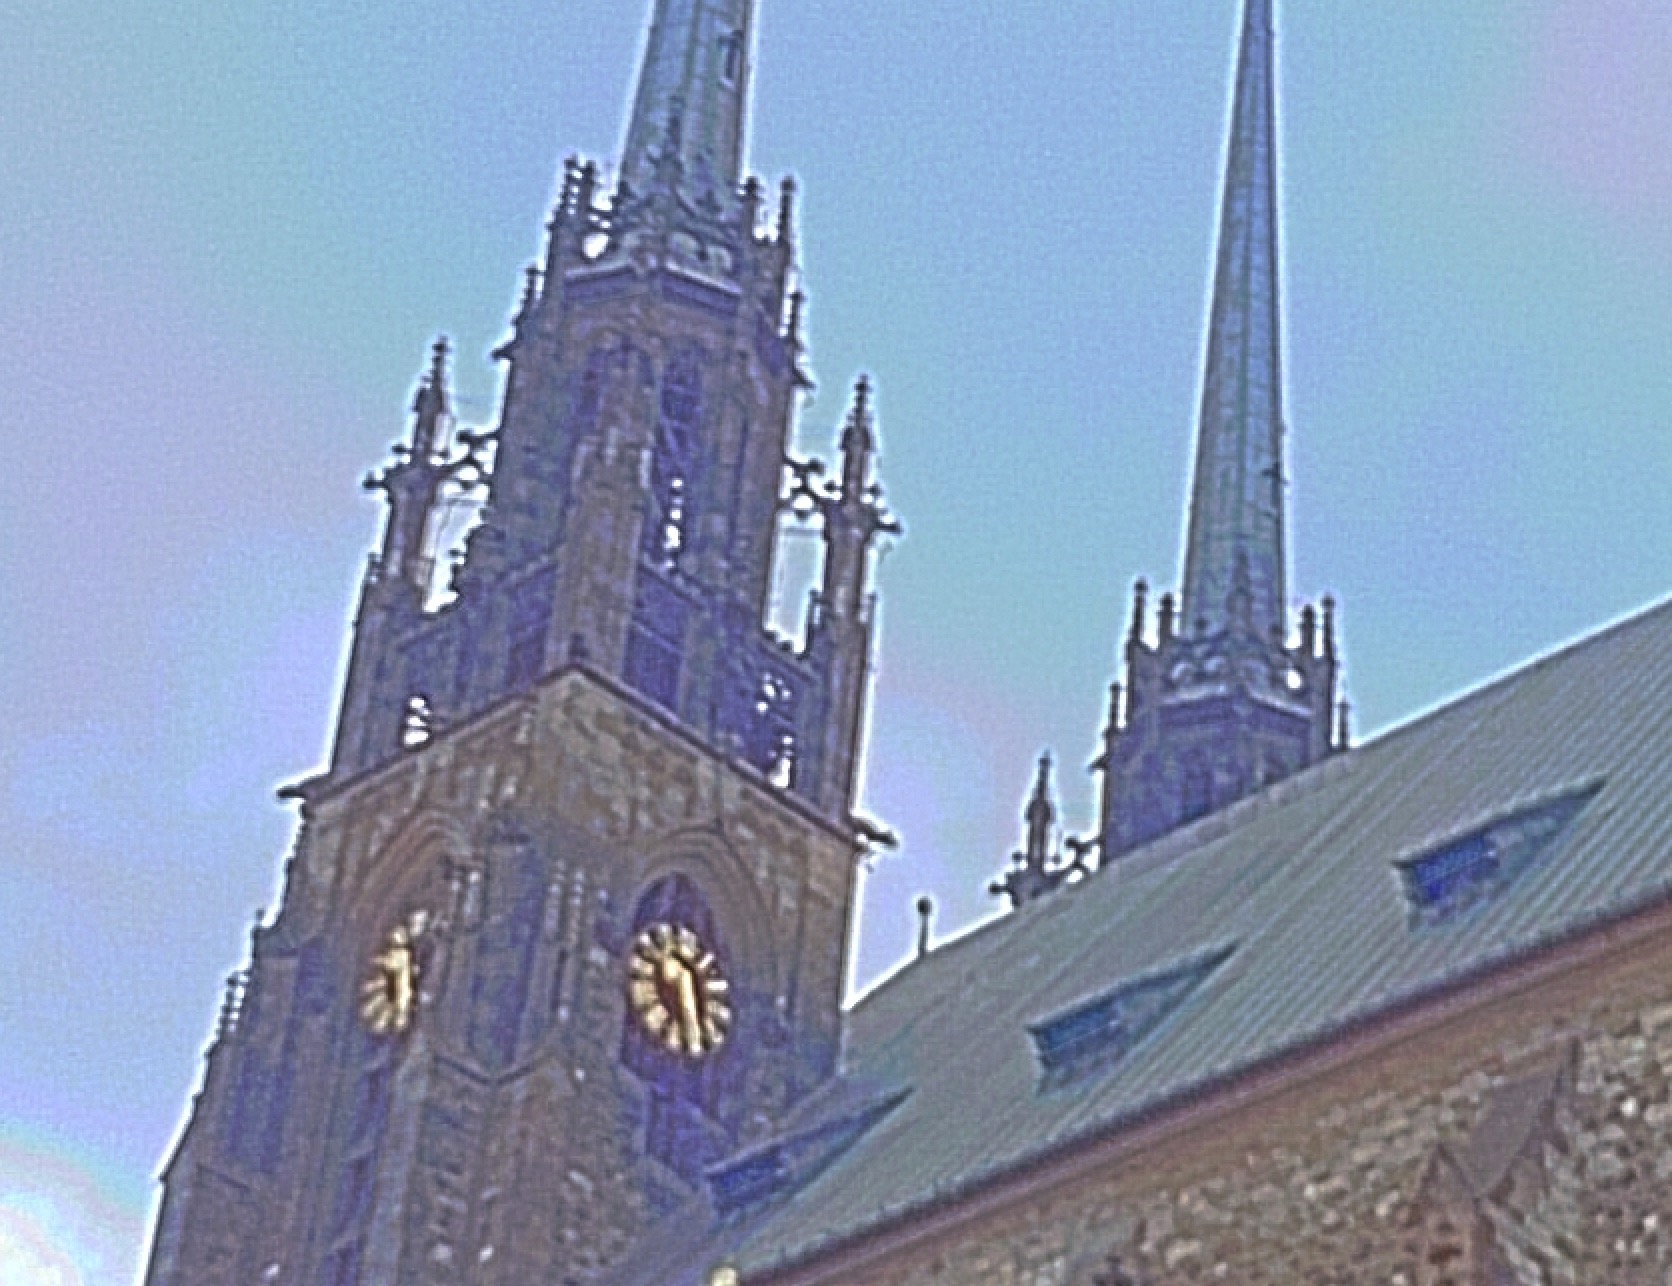
\includegraphics[width=0.35\linewidth]{tmo/durHalo1}
	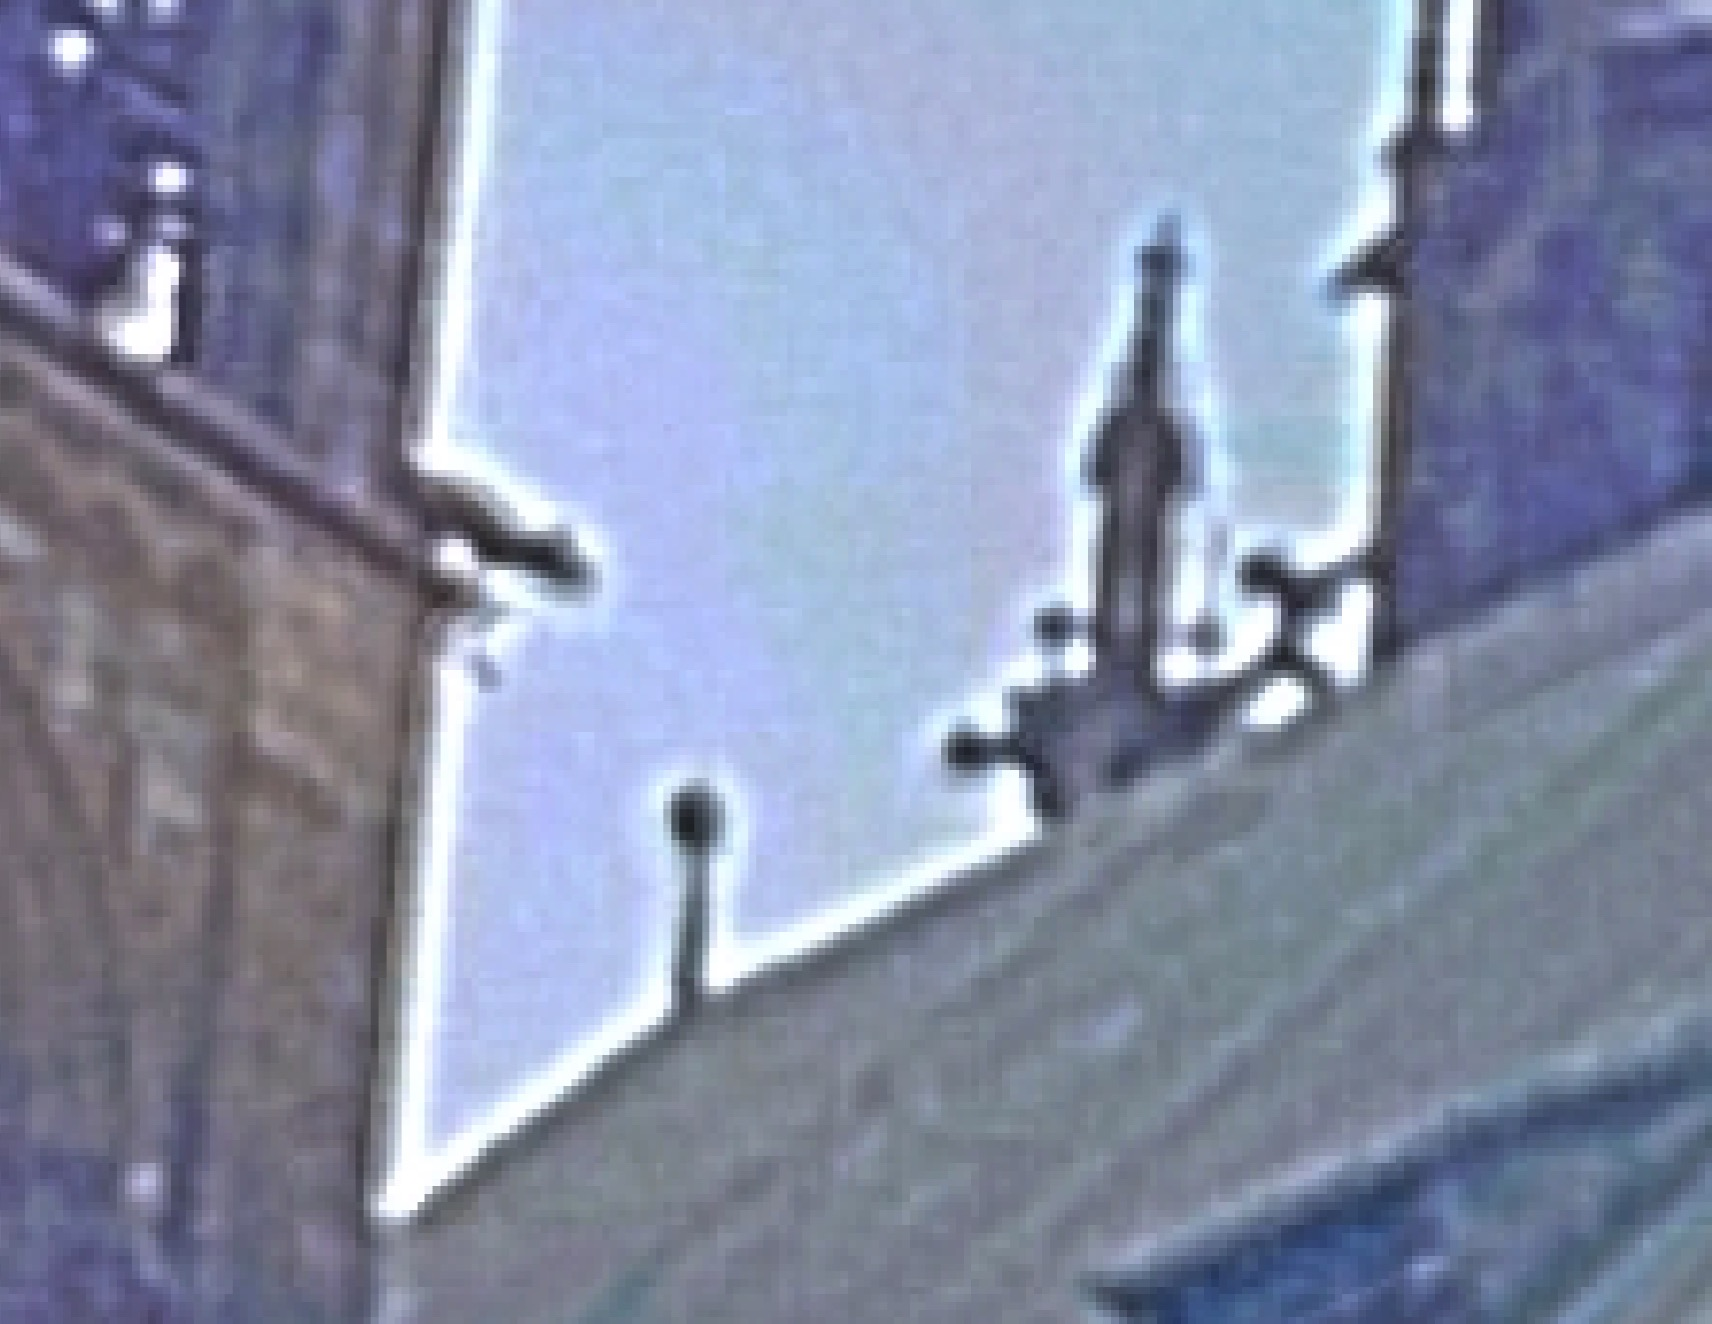
\includegraphics[width=0.35\linewidth]{tmo/durHalo2}
  \caption{Halo efekt}
  \label{fig:DurandHalo}
\end{figure}

%--------------------------------------------------------
\subsection{Porovnania s existujúcimi aplikáciami}
\label{sec:Result-Apps}

Z prieskumu aplikácií boli vybrané užívateľmi naj- lepšie hodnotené riešenia, ktorými bola zachytená scéna \textit{brana}.

\begin{figure}[t]
  \centering
	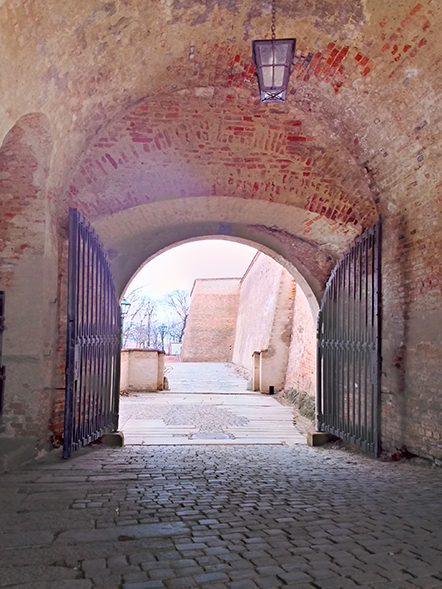
\includegraphics[width=0.24\linewidth]{apps/hdrCamera}
	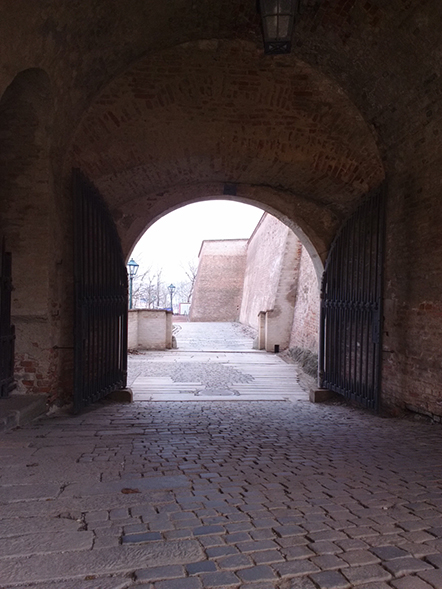
\includegraphics[width=0.24\linewidth]{apps/hdrHq}
	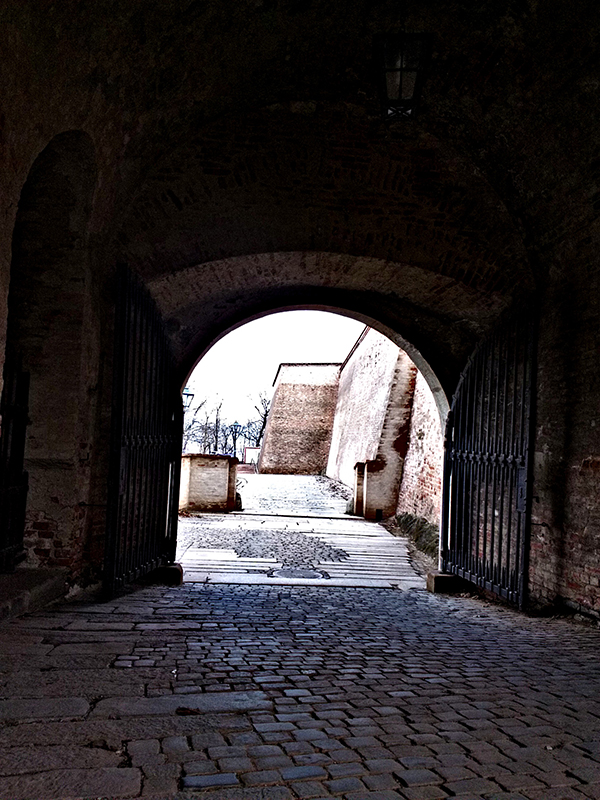
\includegraphics[width=0.24\linewidth]{apps/hdrMax}
	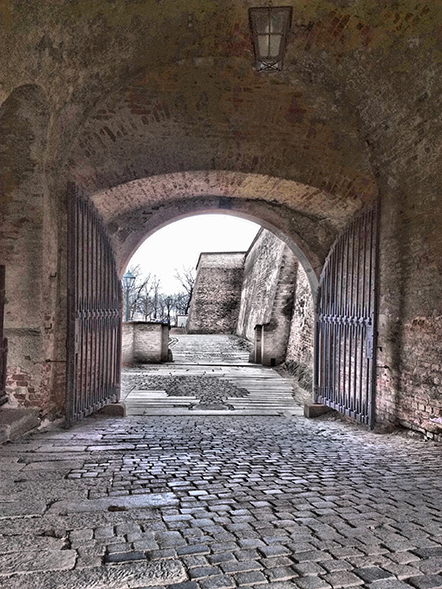
\includegraphics[width=0.24\linewidth]{apps/ultimateHdrCamera}
  \caption{Scéna brány zachytená voľne dostupnými HDR aplikáciami \textit{(z ľava: HDR Camera, HDR HQ, HDR Max, Ultimate HDR Camera)}}
  \label{fig:Apps}
\end{figure}

Začneme najzaujímavejším výsledkom, ktorý vytvorila aplikácia Ultimate HDR Camera.
Na tomto obrázku môžeme vidieť jasného zástupcu fotografií, ktoré si užívateľ predstavuje pod pojmom
"HDR fotografia". Okrem umeleckého zážitku, ktorý výsledná fotografia ponúka zvýraznením detailov
a farieb, môžeme vidieť, že fotografia kvalitne zobrazuje svetlé aj tmavé oblasti scény. To znamená,
že vytvára viacero snímok s~dostatočným rozsahom expozičného času. Z výsledku je rozpoznateľné, že sa jedná
o lokálny operátor, ktorý okrem mapovania tónov pracuje aj s farbami a kontrastom fotografie. Podobný
výsledok by sa nám pravdepodobne nepodarilo dosiahnúť v našej aplikácii, avšak treba poznamenať,
že ani jedna z fotografií \ref{fig:Apps} nemá dostatočný dynamický rozsah na to, aby nepreexponovala
oblohu v pozadí. Vo výsledkoch našej aplikácie sú vo všetkých operátoroch zachované farby oblohy.

Aplikácia HDR Camera ponúka taktiež uspokojivý výsledok, z ktorého možno usúdiť,
že zahŕňa dostatočný dynamický rozsah scény a je použitý lokálny operátor. Pri bližšom pohľade však vidíme,
že na obrázku sa nachádzajú škvrny - miesta, na ktorých sa stráca farebnosť. Príčina tohoto javu však nie je
objasnená. Podobný výsledok sme schopný v našej aplikácii dosiahnúť Durandovým operátorom.

Aplikácie HDR HQ a HDR Max sú príkladom riešení, ktoré nezachytávajú väčší dynamický rozsah scény, ale snažia
sa vytvoriť HDR efekt pomocou filtra.

%--------------------------------------------------------
\subsection{Časová a priestorová zložitosť aplikácie}
\label{sec:Result-Computation}

V rámci analýzy časovej a priestorovej zložitosti sa porovnávala rýchlosť a pamäťová náročnosť jednotli- vých krokov
procesu vytvárania HDR fotografie z~rôz- neho počtu snímok. Hodnoty zložitosti pri vytváraní 5 snímok sú stručne uvedené
v tabuľke \ref{tab:ResultTable}.

\begin{table}[t]
	\vskip6pt
	\caption{Výsledky meraní}
	\centering
	\begin{tabular}{l r}
		\toprule
		 & 5 vytvorených snímok \\
		\midrule
		Snímanie & 1 050 ms / 100 MB \\
		Generovanie HDR & 38 285 ms / 312 MB \\
		Generovanie HDR (OpenCV) & 8 349 ms / 218 MB \\
		Operátor Mantiuk & 1 299 ms \\
		Operátor Reinhard & 1 524 ms \\
		Operátor Durand & 1 423 ms \\
		Operátor Drago & 1 234 ms \\
		Zmenšenie náhľadového obr. & \textless 15 ms \\
		Operátor Durand (náhľad) & 72 ms \\
		Načítanie HDR & 400 ms \\
		Ukladanie HDR & 1200 ms \\
		\bottomrule
	\end{tabular}
	\label{tab:ResultTable}
\end{table}

Merali sa časy a alokovaná pamäť nielen celkov, ale aj ich podproblémov. Pri generovaní HDR obsahu sme sa zamerali
na výber vzoriek pixelov, získavanie krivky odozvy a vytváranie funkcie žiarenia. Vo vlastnej implementácii algoritmu
na generovanie HDR obsahu najviac času spotrebovalo vytvorenie výslednej matice (okolo 15 sekúnd), použiteľnej
pre ďalšie kroky vykonávané knižnicou OpenCV. Vidíme, že knižnica OpenCV má dostatočne optimalizovaný algoritmus
so~skoro polovičnou spotrebou pamäte. Ďalej si môže- me všimnúť, že aplikovanie operátora mapovania tónov na zmenšený
obrázok nám ušetrilo dostatok času na to, aby užívateľ videl výsledok v reálnom čase pri zmene vstupných parametrov.

%--------------------------------------------------------
\subsection{Spätná väzba užívateľov}
\label{sec:Result-Feedback}

Testovania intuitívnosti a estetickosti užívateľského rozhrania sa účastnilo 81 osôb rôznej vekovej kategórie. Užívateľom
bolo poskytnuté zariadenie s aplikáciou a následne boli požiadaní o vyplnenie krátkeho dotazníka. Odpovede na povinné otázky
s možnosťami výberu z \textit{áno} alebo \textit{nie} sú uvedené v tabuľke \ref{tab:FeedbackTable}.

Dizajn aplikácie má pozitívne hodnotenia, ale užívatelia by privítali primerane záživnejšie a farebnejšie rozhranie.

Najviac pripomienok mali užívatelia k tlačítkam v dolnom menu vybraného operátora. Aj napriek snahe vytvoriť ikony,
najlepšie zobrazujúce svoju funkciu, je potrebné mať v aplikácii dialógové okno vysvetľujúce význam jednotlivých
prvkov užívateľského rozhrania.

Ďalšie ohlasy boli venované tlačítku pre zmenu o- rientácie obrázkov. Východzia orientácia náhľadového obrázku sa bude získavať
z metadát súboru a tlačítko bude použiteľné v prípadoch, ak by užívateľovi aktuálne otočenie náhľadového obrázku nevyhovovalo.

V rámci porovnania aplikácie s existujúcimi rieše- niami, citujem odpoveď jedného respondenta:
\begin{quote}
	\textit{Aj napriek tomu, že aplikácia nesleduje najnovšie trendy mobilného dizajnu alebo pravidlá material
	designu, myslím, že je spracovaná lepšie ako veľký počet aplikácií v obchode Google Play.}
\end{quote}

\begin{table}[t]
	\vskip6pt
	\caption{Hodnotenie užívateľského rozhrania}
	\centering
	\begin{tabular}{l c c}
		\toprule
		Otázka & Áno & Nie \\
		\midrule
		Stretli ste sa už s pojmom HDR? & 51.9\% & 48.1\% \\
		Využívate HDR funkcie \\iných zariadení? & 38.3\% & 61.7\% \\
		Zdá sa Vám aplikácia prehľadná? & 96.3\% & 3.7\% \\
		Viete intuitívne, ako pracovať\\s aplikáciou? & 75.3\% & 24.7\% \\
		Reaguje aplikácia plynulo \\na vaše podnety? & 86.4\% & 13.6\% \\
		Má aplikácia estetický \\a minimalistický dizajn? & 88.9\% & 11.1\% \\
		\bottomrule
	\end{tabular}
	\label{tab:FeedbackTable}
\end{table}

%--------------------------------------------------------
%--------------------------------------------------------
\section{Záver}
\label{sec:Conclusion}

Primárnym cieľom práce je oboznámenie sa s problematikou spracovania HDR obrazu a následný návrh 
a~implementácia mobilnej aplikácie pre akvizíciu, spracovanie, zobrazenie a úpravu HDR fotografií.
V teoretickej časti sú zhrnuté znalosti nadobudnuté štúdiom odporúčanej literatúry a internetových
zdrojov o aktuál- nych problémoch spracovania HDR a metódach ich riešenia. V zdrojovom kóde mobilnej 
aplikácie je rozpracovaný a zdokumentovaný postup tvorby HDR fotografie.

Výsledná analýza preukázala, že aj napriek množ- stvu mobilných aplikácií s rozmanitou funkcionalitou
existuje priestor pre aplikácie, ktoré by ponúkali lepšie riešenie alebo užívateľsky prívetivejšie
prostredie. Úče- lom je užívateľovi ponúknuť rozhranie s funkciami, ktoré potrebuje a dokáže sa v aplikácii
ľahko a intuitívne pohybovať.

Táto práca položila základ pre vývoj prepracovanejších metód, ktoré možno v budúcnosti vytvoria komplexnú
mobilnú aplikáciu s využiteľnosťou pre širokú škálu užívateľov.

\section*{Poďakovanie}
Rád by som poďakoval pánovi docentovi Ing. Martinovi Čadíkovi, Ph.D. za odbornú pomoc, pripomienky a rady
poskytnuté počas tvorby tejto práce.

%--------------------------------------------------------
%	REFERENCE LIST
%--------------------------------------------------------
\phantomsection
\bibliographystyle{unsrt}
\bibliography{2018-ExcelFIT-HDRapp-bib}

%--------------------------------------------------------
\end{document}